\documentclass[12pt,a4paper]{article}
\usepackage[utf8]{inputenc}
\usepackage[spanish]{babel}
\usepackage{amsmath}
\usepackage{amsfonts}
\usepackage{amssymb}
\usepackage{makeidx}
\usepackage{graphicx}
\usepackage[left=2cm,right=2cm,top=2cm,bottom=2cm]{geometry}

\author{Felipe Alvarado Galicia}
\title{MÉTODOS GEOMÉTRICO, ALGEBRAICO Y DESACOPLO CINEMÁTICO}
\date{Profesor:Carlos Enrique Moran Garabito\\
Materia: Cinematica de Robots\\
22 de octubre de 2019}

\begin{document}
\maketitle
 
\includegraphics[scale=1]{logo1.png}\\
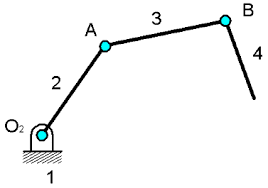
\includegraphics[scale=1]{imag5.png} 
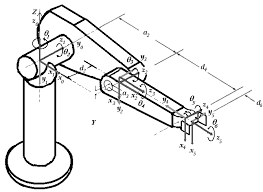
\includegraphics[scale=1]{imag8.png}\\\\\\\\\\\\\\\\\\\\\\\\\\\\\\\\\\\\\\\\\\\\\\

\tableofcontents

\section{CINEMÁTICA DE POSICIÓN
}
Para entrar en el tema de los metodos que queremos conocer, debemos antes empaparnos un poco e introducirnos al inicio, que es la misma cinematica de posición.\\\\

La cinemática del robot estudia el movimiento del mismo con respecto a un sistema de referencia fijo
sin considerar considerar las fuerzas fuerzas
y momentos momentos que originan originan
dicho movimiento.\\
Se divide en dos por asi decirlo, que son la inversa y la directa:\\

\subsection{Cinemática DIRECTA}
Determina la localización del
extremo del robot, con respecto a un sistema de
coordenadas de referencia, conocidos los valores de las articulaciones y los parámetros geométricos de los elementos de robot.\\
\subsection{Cinemática INVERSA}
Conocida la configuración del robot determina cual debe ser la configuración del robot(articulaciones y parametros geométricos).\\

Desde el punto de vista de la robótica, el
problema cinemático inverso es más complejo.\\\\

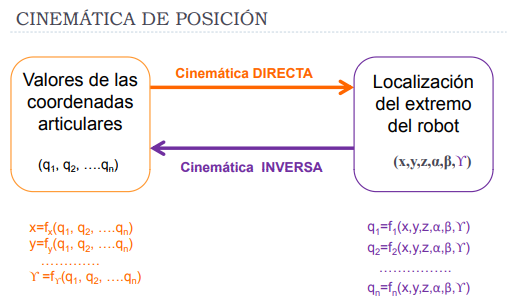
\includegraphics[scale=1.2]{1.PNG} \\\\\

Una de las formas que existen para abordar el problema cinematico directo es el geometrico.\\
\subsubsection{Métodos geometricos}
Los métodos geométricos permiten tener normalmente los valores de las primeras variables articulares, que son las que consiguen posicionar el robot.\\
El procedimiento se basa en encontrar un número suficiente de relaciones geométricas en las que intervendrán las coordenadas del extremo del robot, sus coordenadas articulares y las dimensiones físicas de sus elementos.\\
Método no sistemático (aplicación limitada a robots con pocos grados de libertad).\\
Utiliza relaciones geométricas para obtener directamente la posición del extremo del robot en función de las variables articulares.\\
Requiere buena visión especial.\\\\
Es un método no sistemático que utiliza las relaciones geométricas para obtener obtener la posición posición del extremo extremo del robot.\\
Normalmente se emplea para la obtención de la posición y no de la orientación.\\
Se usan en robots de pocos grados de libertad.\\
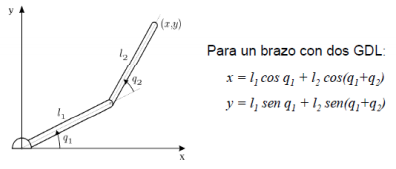
\includegraphics[scale=1.5]{2.PNG} \\
Existe un método sistemático para situar los sistemas de coordenadas asociados a cada eslabón y obtener la cadena cinemática del robot.
Método de Denavit-Hatenberg (1955).\\
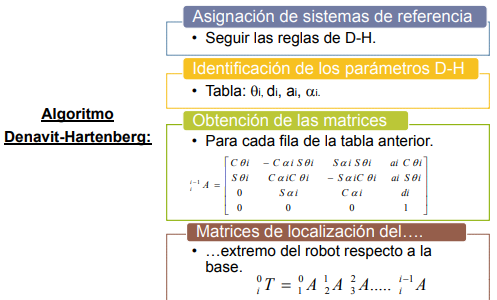
\includegraphics[scale=1]{D-H.PNG} \\
\subsection{CINEMÁTICA INVERSA}
\subsubsection{Desacoplo cinemático}
En general no basta con posicionar el extremo del robot en un punto del espacio, sino que es preciso conseguir que la herramienta se oriente de una manera determinada.\\
Para ello, los robots cuentan con otros tres grados de libertad adicionales, situados al final de la cadena cinemática y cuyos ejes, generalmente, se cortan en un punto, que informalmente se denomina muñeca del robot.\\
Si bien la variación de estos tres últimos grados de libertad origina un cambio en la posición final del extremo real del robot, su verdadero objetivo es poder orientar la herramienta del robot libremente en el espacio.\\
El método de desacoplo cinemático saca partido de este hecho, separando ambos problemas: Posición y orientación.\\



\paragraph{binliografia}
http://www.kramirez.net \\
https://ocw.ehu.eus/pluginfile.php \\


\end{document}